\paragraph{Behavioral Cloning (BC). [MAX 5]} \mbox{} \\ 
Behavioral Cloning is one of the first approaches used to learn a task from a set of demonstrations. It is framed as a Supervised Learning problem, solved through Algorithm \ref{alg:bc}. In this setting there are at least to questions to answer: 
\begin{enumerate*}[label=\textbf{(\arabic*)}]
    \item Choose whether to optimize in trajectory space or action space.  
    \item What kind of representation to use for the policy.
\end{enumerate*}
Generally speaking, Algorithm \ref{alg:bc} defines the procedure used to solve the learning task, given the dataset $D^{E}$, a parameterized learner policy $\pi^{L}_{\theta}$, and a loss-function $\mathcal{L}$, the goal is to find the policy parameter that minimizes the loss-function, in other terms, $\theta^{*} = \underset{\theta}{argmin} \ \mathbb{E}_{(\boldsymbol{\tau}, \mathbf{c}) \sim D^{E}} \ [\mathcal{L}((\boldsymbol{\tau}, \mathbf{c}), \ \pi^{L}_{\theta})]$.
\newline According to \cite{osa2018algorithmic,zheng2021imitation_progress_taxonomies_opportunities}, BC methods can be categorized as Model-Free and Model-Based, and based on the fact that the policy is optimized either in the trajectory space or in the action space.
\begin{algorithm}
\caption{Abstract Algorithm for Behavioral Cloning}\label{alg:bc}
\begin{algorithmic}
\Require A set of expert demonstrations $\mathcal{D}^{E}$, a parameterized policy $\pi_{\theta}^{L}$
\Ensure The optimal set of policy parameter $\theta^{*}$
\State Optimize $\mathcal{L}$ w.r.t. policy parameter $\theta$ using $\mathcal{D}^{E}$
\end{algorithmic}
\end{algorithm} 

\textbf{Model-Free methods} learns a policy that reproduces the expert's behavior without learning/estimating system dynamics. Since they do not require neither to estimate the system dynamic nor to learn a reward function, they are simple to implement and do not necessary require system  interactions. 

Model-Free methods that derive policy in the space of trajectories were very popular in the context of Model-Free BC for robotic manipulation trajectory planning, given their ability to explicitly model constraints on the generated trajectory (e.g. a smooth convergence to the goal state). Indeed, in this setting very popular and studied methods are the \textit{Dynamic Movement Primitives} (DMPs) \cite{ijspeert2002learning,ijspeert2013dynamical}, and the \textit{Probabilistic Movement Primitives} (ProMPs) \cite{}. \textcolor{red}{[To continue...]}

Regarding the methods that derive the policy in the action-space. One of the primal work is such setting was \cite{pomerleau1988alvinn}, which proposed \textit{ALVINN}, an autonomous vehicle driving system based on a Neural Network, that infers the steering angle, given a camera image as input. The network was trained on pairs (image, steering-angle), the steering-angle was discretized over 45 units, and the training was defined as a supervised classification problem. This work immediately emphasized the problem of compounding-error, caused by covariate-shift phenomena. This issue occurs because an action $a_{t}$ influences the next state $s_{t+1}$, violating the i.i.d assumption of Supervised Learning, and generating a test-data distribution, that may be different from the the training one. This phenomena has a relevant consequence on the expected performance of the system. Indeed, assuming to have a system that makes an error with probability $\epsilon$, and a task with time-horizon $T$, then, due to compounding error, a supervised learner reaches a total cost of $O(\epsilon \ T^{2})$, rather than $O(\epsilon \ T)$ \cite{ross2010efficient_reductions,ross2011dagger}. To attenuate this problem, interactive supervised learning algorithms have been proposed, such as the well-known \textit{DAgger} \cite{ross2011dagger}. Algorithm \ref{alg:dagger} describes the DAgger procedure. It is an aggregation strategy, based on the idea to train the policy $\pi$ under the state-distribution induced by the policy itself, but with the correct action performed by the expert. the main problem with DAgger is that it requires the expert to interact with the system during the training, introducing both safety and data-efficiency problems, especially when the system does not provide the human expert with sufficient control authority during the sampling process \cite{laskey2017comparing_hc_rc}. \begin{algorithm}
\caption{DAgger Algorithm \cite{ross2011dagger}}\label{alg:dagger}
\begin{algorithmic}
\Require Initial Dataset $D \leftarrow \emptyset$, Initial policy $\pi^{L}_{1}$
\Ensure The best policy $\pi^{L}_{i}$
\For {$i=1, \dots N$}
    \State Sample $T-step$ trajectories using $\pi^{L}_{i}$
    \State Let $D_{i} = {(s_{t}, \pi^{E}(s_{t}))}$, state $s_{t}$ visited by policy $\pi^{L}_{i}$, 
    \State and actions given by the expert
    \State Aggregate Dataset, $D \leftarrow D \bigcup D_{i}$
    \State Train policy $\pi^{L}_{i}$ on $D$
    \State Let $\pi^{L}_{i+1} = \beta_{i}\pi^{E} + (1- \beta_{i})\pi^{L}_{i}$
\EndFor
\end{algorithmic}
\end{algorithm}
\newline Human-Guided DAgger (HG-DAgger) \cite{kelly2019hg_dagger} is an extension of the classic DAgger strategy, in which the human expert observes the rollout of the current policy, so if the agent has entered an unsafe region of the state space, the expert takes control and guides the system to a safe and stable region. In \cite{jang2022bc_z} was shown how HG-DAgger can be effectively used in the context of robotic manipulation. Indeed, starting from the same total number of episodes, a policy trained with only expert demonstration has a significantly lower success rate than a policy trained on a dataset with both expert demonstration and expert adjustments. In the context of Interactive Learning for Robot Manipulation, other works of interest include \cite{mandlekar2020human_in_the_loop,chisari2022correct}. In \cite{chisari2022correct}, a human expert provides both corrective and evaluative feedback. %(Figure \ref{fig:feedback}).
The former consists in the human that takes control of the robot to adjust the trajectory, the latter consists in a scalar weight $q$, set to 1 if the trajectory is satisfactory, 0 the trajectory is not satisfactory, $\alpha$ if the trajectory is adjusted by the expert, where $\alpha$ is the ration between non-corrected and corrected samples. Then a Neural Network % in Figure \ref{fig:architecture}
was trained by minimizing a weighted version of the maximum-likelihood $\mathcal{L}(a_{t},s_{t}) = - q \ log(\pi^{L}_{\theta}(a_{t}|s_{t}))$. Real-world experiments show that with a training time of \textbf{41 minutes}, including environmental reset, it is possible to have an agent capable of performing tasks such as picking up a cube or pulling a plug.
%\begin{figure}[htbp]
    \begin{subfigure}{0.45\textwidth}
         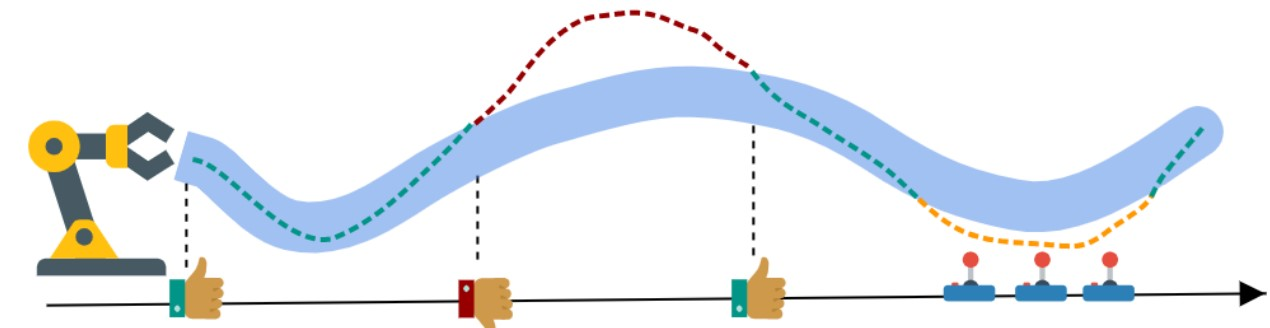
\includegraphics[width=\textwidth]{Figures/images/correct-me-if-i-am-wrong/feedback.jpg}
         \caption{Evaluative feedback: the expert labels the sub-trajectory as satisfactory or not. Corrective feedback: the human guides the robot towards the correct trajectory}
         \label{fig:feedback}
    \end{subfigure}
    \hfill
    \begin{subfigure}{0.50\textwidth}
         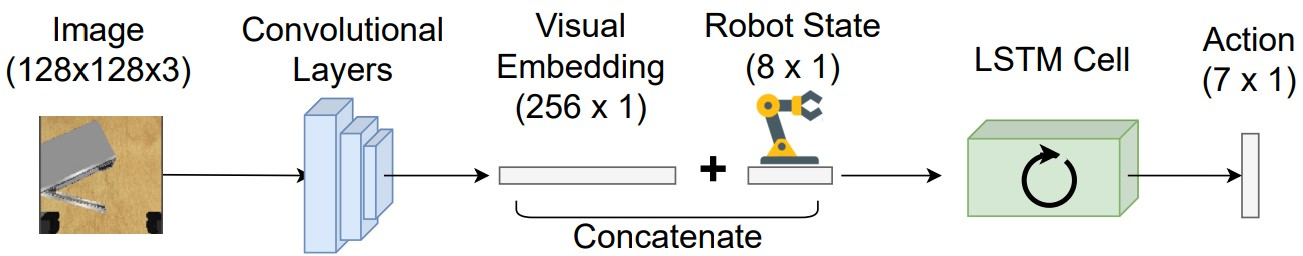
\includegraphics[width=\textwidth]{Figures/images/correct-me-if-i-am-wrong/correct_me_architecture.jpg}
         \caption{Policy architecture: The input is an RGB image of the scene, the output is the desired end-effector pose and the gripper state}
         \vspace{0.5cm}
         \label{fig:architecture}
    \end{subfigure}
    \caption{(\ref{fig:feedback}) Representation of the meaning of the feedback, (\ref{fig:architecture}) Policy architecture proposed in \cite{chisari2022correct}}
    \label{fig:correct_me_if_im_wrong}
\end{figure}

%Classic Behavioral Cloning

Despite the covariate-shift problem, \cite{zhang2018deep_vr_teleoperation} showed that very interesting performance can be obtained in the context of Robot Manipulation Task, by means of Behavioral Cloning and high quality demonstrations given by teleportation system. In this work, a CNN was trained to predict the desired linear-velocity and angular-velocity of the end-effector, with the binary gripper state (open/close), given in input the current RGB-D observation of the scene, and the position of three points of the end-effector, during the last 5 time-steps. The system was tested on 10 tasks, and the performance are reported in Table \ref{table:deep_vr_teleoperation_results}.
\begin{table}
\centering
\caption{Statistics of Training set, and Test Success rate \cite{zhang2018deep_vr_teleoperation}}
\label{table:deep_vr_teleoperation_results}
\resizebox{\linewidth}{!}{%
\begin{tabular}{c|c|c|c|c|c|c|c|c|c|c}
task                                                                                                                                   & reaching & grasping & pushing & plane & cube & nail & grasp-and-place & grasp-drop-push & grasp-place-x2 & cloth  \\ 
\hline
\rowcolor[rgb]{0.753,0.753,0.753} \#demo                                                                                               & 200      & 180      & 175     & 319   & 206  & 215  & 109             & 100             & 60             & 100    \\ 
\hline
\begin{tabular}[c]{@{}c@{}}demo duration \\(min)\end{tabular}                                                                          & 13.7     & 11.1     & 16.9    & 25.0  & 12.7 & 13.6 & 12.3            & 14.5            & 11.6           & 10.1   \\ 
\hline
\rowcolor[rgb]{0.753,0.753,0.753} \begin{tabular}[c]{@{}>{\cellcolor[rgb]{0.753,0.753,0.753}}c@{}}Test success rate\\(\%)\end{tabular} & 91.6     & 97.2     & 98.9    & 87.5  & 85.7 & 87.5 & 96.0            & 83.3            & 80.0           & 97.4  
\end{tabular}
}
\end{table}
% Meta-Learning, few shot, zero-shot. Il problema principale è che per l'esecuzione di differenti task c'è bisogno di riaddestrare da zero le policy
\newline One important aspect to note is that for each task the network was trained from scratch. This is not a desired property for a highly adaptable system, as stated in Section \ref{sec:intro}. For this reason, methods based on Meta-Learning algorithms have been proposed. The idea behind Meta-Learning is to train a model on a variety of tasks, in such a way that it can solve a new tasks, using only a small number of training samples \cite{finn2017maml}. Algorithm \ref{alg:maml} describes the steps followed by the \textit{Model-Agnostic Meta-Learning} (MAML) algorithm \cite{finn2017maml}, that is the base for different methods which apply One-shot Imitation Learning in the context of Behavioral Cloning \cite{finn2017one_shot_visual_il,yu2018daml,yu2018one_shot_hil}.\begin{algorithm}[h]
\caption{Model-Agnostic Meta-Learning (MAML) \cite{finn2017maml}}
\label{alg:maml}
\begin{algorithmic}
\Require Distribution over tasks $p(\mathcal{T})$
\State Randomly initialize $\theta$
\While {$i=1, \dots N$}
    \State Sample batch of tasks $ \mathcal{T}_{i} \sim p(\mathcal{T})$
    \For {\textbf{all} $\mathcal{T}_{i}$}
        \State Evaluate $\nabla_\theta \mathcal{L}_{\mathcal{T}_{i}}(f_{\theta})$ w.r.t. $K$ examples
        \State Compute adapted parameters with gradient descent: $\theta'_{i} = \theta - \alpha \nabla_\theta\mathcal{L}_{\mathcal{T}_{i}}(f_{\theta})$
    \EndFor
    \State Update $\theta \leftarrow \theta - \beta \nabla_\theta \sum_{\mathcal{T}_{i} \sim p(\mathcal{T})} \mathcal{L}_{\mathcal{T}_{i}}(f_{\theta'_{i}})$
\EndWhile
\end{algorithmic}
\end{algorithm}
\newline In \cite{finn2017one_shot_visual_il}, MAML algorithm was used to prove the effectiveness of Meta-Learning in the context of real robot manipulation, with visual observations, as opposite to \cite{duan2017one_shot_il}. A CNN was trained by following the Algorithm \ref{alg:maml}, using as loss-function the Mean Squared Error, computed between the predicted action and the ground truth one. For real-robot experiments a dataset of 1300 placing demonstrations (i.e. place an holded object in a target container), containing near to 100 different objects, was collected through teleportation. The trained system was tested by performing the adaptation step on one video demonstration, over 29 new objects, moreover, between the video demonstration and the actual execution, the objects configuration was changed. In this setting the system reached the $\mathbf{90\%}$ of success rate, outperforming baseline methods based on LSTM \cite{duan2017one_shot_il}, and contextual network (i.e. a CNN that takes in input the current observation and the image representing the target state).
\newline In \cite{yu2018daml}, the \textit{Domain Adaptive Meta-Learning} algorithm (DAML) was proposed with the goal of learning to infer a policy from a single human demonstration. To achieve it, a two-step algorithm was proposed. In the first-step, called \textbf{Meta-Learning step}, given in input, for each task $\mathcal{T}$, a set of human demo $D^{h}_{\mathcal{T}}$ and a set or robot demo $D^{r}_{\mathcal{T}}$ (Figure \ref{fig:daml}), the \textit{initial policy parameters} $\theta$ and the \textit{adaptive loss} parameters $\psi$ are learned, solving the problem in Formula \ref{eq:daml}. \begin{equation}
 \label{eq:daml}
 \underset{\theta,\psi}{\min} \sum_{\mathcal{T} \sim p(\mathcal{T})} \sum_{\mathbf{d}^{h} \sim D^{h}_{\mathcal{T}}} \sum_{\mathbf{d}{^r} \sim D^{r}_{\mathcal{T}}} \mathcal{L}_{BC}(\theta - \alpha \nabla_\theta\mathcal{L}_{\psi}(\theta,\mathbf{d}^{h}), \mathbf{d}^{r})
\end{equation}

\newline Where the outer loss is $\mathcal{L}_{BC}(\phi,\mathbf{d^{r}}) = \sum_{t} log(\pi_{\phi}(a_{t}|s_{t},o_{t}))$, and the inner-loss $\mathcal{L}_{\psi}$, is the learned adaptive loss, which is used during the \textbf{Meta-Test step}, where the policy parameters are adapted with gradient descent given in input a video of human demo of a new task $\mathcal{T}$, i.e. $\psi_{\mathcal{T}} = \theta - \alpha \nabla_{\theta} \mathcal{L}_{\psi}(\theta, \mathbf{d^{r}})$. Experimental evaluation on tasks such as placing, pushing, and pick-and-place, has shown that: \begin{enumerate*}[label=\textbf{(\alph*)}]
    \item The system was able to generalize across both new objects and objects configuration starting from only a single human-demonstration.
    \item A performance degradation was observed in large domain-shift experiments, such as novel backgrounds and different camera view-points.
\end{enumerate*}
The work proposed in \cite{yu2018one_shot_hil} is an extension of DAML, for multi-stage tasks, i.e. tasks that are composed of different motion primitives. \begin{figure}[htbp]
    \centering
    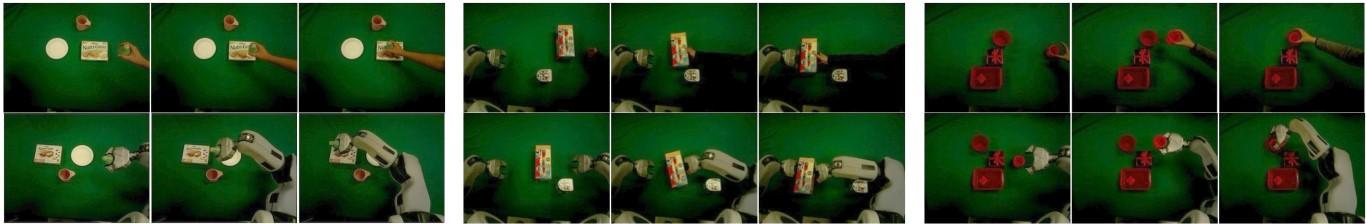
\includegraphics[width=\textwidth]{Figures/images/daml/tasks.jpg}
    \caption{Tasks performed in \cite{yu2018daml}. (Top row) Human demonstration, (Bottom row) robot demonstration. (Left) Placing task, (Middle) pushing task, (Right) pick-and-place task.}
    \label{fig:daml}
\end{figure}


Generally speaking, all the works described up to now, consider the task distribution $p(\mathcal{T})$ as composed of one-single task, but with many different variations \cite{finn2017one_shot_visual_il} or different, but related tasks \cite{yu2018daml}. Very recent methods try to generalize BC to a huge variety of tasks \cite{jang2022bc_z,mandi2022towards_more_generalizable_one_shot}, 
In \cite{jang2022bc_z}, a large-scale dataset containing \textbf{100} diverse manipulation tasks was collected. The demonstrations were collected through expert teleoperation and shared autonomy process (DAgger \cite{ross2011dagger}). The demonstrated tasks were related to pick-and-place, grasp, pick-and-drag, pick-and-wipe, and push skills. The dataset was used to train the network in Figure \ref{fig:bcz_architecture}. As it can be noted the samples were composed by current robot observation, and a conditioning represented by either a vocal command or a video demo. The idea was that training a conditioned policy over the current observation $o_{t}$, and a task representation $c_{t}$, $\pi^{L}(a_{t}|o_{t}, c_{t})$, it would allow the policy to generalize over new tasks in a zero-shot manner (i.e. without any fine-tuining). Experimental results shown that, over 28 held-out tasks, containing both completely new object, and known objects but in different tasks, an average success rate of \textbf{38\%} was reached in the easiest setting, with only one distractor and with language conditioning. The success rate dropped to \textbf{4\%} in the hardest setting with 4 distractors and video conditioning. These bad performance can be justified by the classic training procedure followed, while different advantages may be gained from Meta-Learning algorithms, and the way in which the human video embedding was obtained, through a CNN on a 4x5 matrix
of images, with a completely loss of temporal information.
\begin{figure}[htb!]
    \centering
    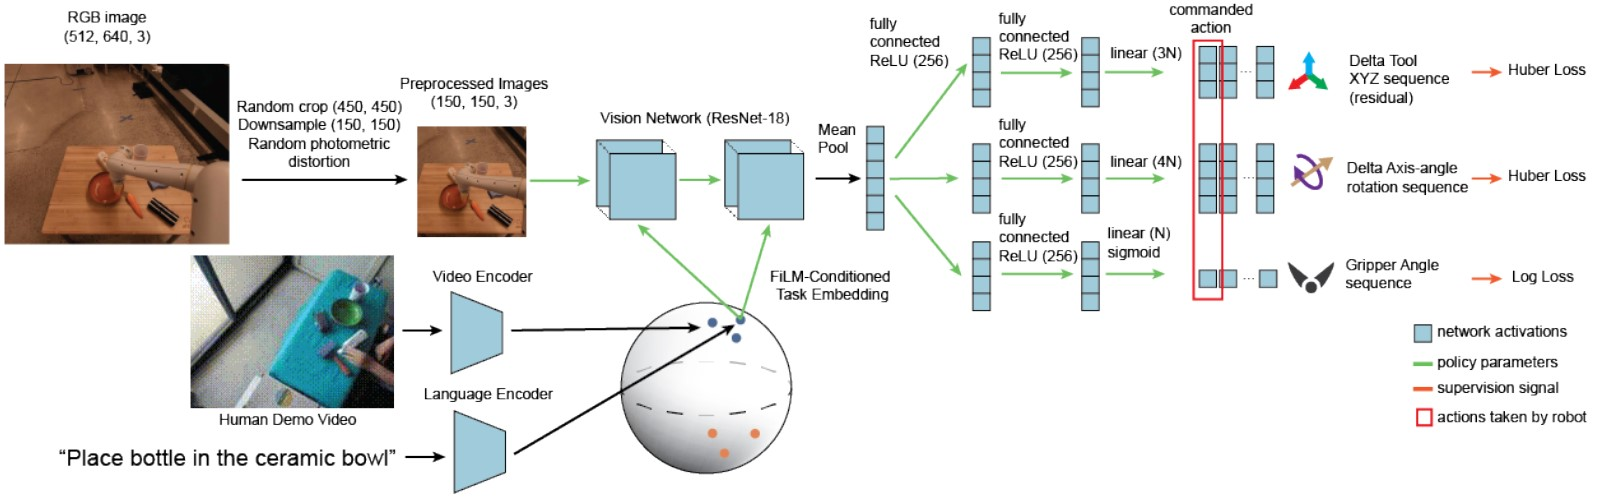
\includegraphics[width=0.9\textwidth]{Figures/images/bc_z/bc-z-network.jpg}
    \caption{Architecture proposed in \cite{jang2022bc_z}}
    \label{fig:bcz_architecture}
\end{figure}


\textbf{Model-Based methods},

